\documentclass[aspectratio=169,11pt]{beamer}
\usetheme{Madrid}
\usepackage[T1]{fontenc}
\usepackage{lmodern}
\usepackage{amsmath,amssymb}
\usepackage{booktabs,tabularx,multicol}
\usepackage{tikz}
\usepackage{pgfplots}
\pgfplotsset{compat=1.17}
\usetikzlibrary{arrows.meta,positioning}

% ---------- colours (same palette as capstone_phase1.tex and 07_compare.py) ----------
\definecolor{navy}{HTML}{1F3A5F}
\definecolor{accent}{HTML}{2A78D6}
\definecolor{warm}{HTML}{EB6834}
\definecolor{aqua}{HTML}{1BAF7A}
\definecolor{gold}{HTML}{EDA100}
\definecolor{soft}{HTML}{EEF3FA}
\definecolor{ink}{HTML}{333333}
% one fixed colour per run
\colorlet{cA1}{accent}
\colorlet{cA2}{warm}
\colorlet{cA3}{aqua}
\colorlet{cA4}{gold}
\setbeamercolor{structure}{fg=navy}
\setbeamercolor{palette primary}{bg=navy,fg=white}
\setbeamercolor{palette secondary}{bg=navy!85!black,fg=white}
\setbeamercolor{palette tertiary}{bg=navy!70!black,fg=white}
\setbeamercolor{frametitle}{bg=navy,fg=white}
\setbeamercolor{title}{bg=navy,fg=white}
\setbeamercolor{block title}{bg=accent,fg=white}
\setbeamercolor{block body}{bg=soft,fg=ink}
\setbeamercolor{block title alerted}{bg=warm,fg=white}
\setbeamercolor{block body alerted}{bg=warm!8,fg=ink}
\setbeamercolor{block title example}{bg=aqua,fg=white}
\setbeamercolor{block body example}{bg=aqua!8,fg=ink}
\setbeamertemplate{navigation symbols}{}
\setbeamertemplate{itemize items}[circle]
\setbeamertemplate{section in toc}[sections numbered]

\newcommand{\code}[1]{\texttt{\small #1}}
\newcommand{\best}[1]{\textbf{#1}}


\title[CS-781 Phase 1: results and next steps]{Phase 1: What A1--A4 Tell Us}
\subtitle{Results of the four architecture runs, and the experiments they motivate}
\author[Manish Kumar]{Manish Kumar (251330604)}
\institute{CS-781, IIT Kanpur}
\date{27 September 2026}

\begin{document}

\begin{frame}
  \titlepage
\end{frame}

\begin{frame}{Outline}
  \begin{multicols}{2}
  \tableofcontents
  \end{multicols}
\end{frame}

% =====================================================================
\section{Setup of the four runs}

\begin{frame}{A controlled comparison: only the architecture changes}
  \begin{columns}[T]
    \begin{column}{0.50\textwidth}
      \footnotesize
      \begin{block}{Shared by all four runs (\code{configs/base.yaml})}
        \begin{itemize}
          \item Legal byte-level BPE, 32k vocabulary.
          \item Mix: SC 30\%, HC 35\%, tribunals 25\%, acts 10\%.
          \item 3000 steps $\times$ 65{,}536 tokens = \textbf{196.6M tokens}.
          \item AdamW, lr $6\!\times\!10^{-4}\to6\!\times\!10^{-5}$ cosine, 200 warm-up steps.
          \item Block 1024; validation loss on the 257 tokens after a 768-token prefix.
          \item Decoding: $\tau{=}0.8$, top-$k$ 50, top-$p$ 0.95, rep.\ penalty 1.1.
          \item One NVIDIA H200 NVL.
        \end{itemize}
      \end{block}
    \end{column}
    \begin{column}{0.46\textwidth}
      \small
      \begin{tabularx}{\textwidth}{@{}lX@{}}
        \toprule
        Run & Design\\
        \midrule
        \textcolor{cA1}{\textbf{A1}} & Decoder-only GPT: learned positions, LayerNorm, GELU, full causal MHA. 8L, $d{=}768$.\\
        \textcolor{cA2}{\textbf{A2}} & Encoder--decoder: bidirectional encoder, cross-attending decoder, sinusoidal. 6+6L, $d{=}640$.\\
        \textcolor{cA3}{\textbf{A3}} & Prefix-LM hybrid: bidirectional prompt + causal continuation, ALiBi. 8L, $d{=}768$.\\
        \textcolor{cA4}{\textbf{A4}} & Efficient decoder: RoPE, RMSNorm, SwiGLU, GQA (4 KV heads), sliding window 256 with global layers 3/6/9. 10L, $d{=}768$.\\
        \bottomrule
      \end{tabularx}
    \end{column}
  \end{columns}
\end{frame}

% =====================================================================
\section{Results}

\begin{frame}{Results at a glance}
  \centering\small
  \begin{tabular}{@{}lrrrrrrrr@{}}
    \toprule
    & \multicolumn{2}{c}{Parameters} & \multicolumn{2}{c}{Validation} & \multicolumn{3}{c}{Dev set (200 prompts)} & \\
    \cmidrule(lr){2-3}\cmidrule(lr){4-5}\cmidrule(lr){6-8}
    Run & total & non-emb & loss & ppl & BERTScore & ROUGE-L & BLEU-4 & GPU h\\
    \midrule
    \textcolor{cA1}{\textbf{A1}} GPT       & 82.1M & 56.7M & \best{2.430} & \best{11.36} & \best{0.8364} & 0.2225 & \best{0.1104} & \best{0.39}\\
    \textcolor{cA2}{\textbf{A2}} Enc--dec  & 89.4M & 68.9M & 3.082 & 21.79 & 0.8154 & 0.1732 & 0.0318 & 0.87\\
    \textcolor{cA3}{\textbf{A3}} Prefix-LM & 81.3M & 56.7M & 2.494 & 12.11 & 0.8349 & 0.2202 & 0.1100 & 0.41\\
    \textcolor{cA4}{\textbf{A4}} Efficient & 87.5M & 62.9M & 2.445 & 11.53 & 0.8346 & \best{0.2234} & \best{0.1104} & 0.75\\
    \bottomrule
  \end{tabular}

  \vspace{4mm}
  \begin{columns}[T]
    \begin{column}{0.47\textwidth}
      \begin{block}{Ranking by validation loss}
        \small A1 $<$ A4 $<$ A3 $\ll$ A2.
        The three single-stack models are within 0.064 nats of each other.
        A2 is 0.65 nats behind.
      \end{block}
    \end{column}
    \begin{column}{0.47\textwidth}
      \begin{alertblock}{Ranking by generation metrics}
        \small A2 is clearly worse: $-0.021$ BERTScore, and a third of the others' BLEU-4.
        A1, A3 and A4 differ by less than 0.002 BERTScore, which on 200 prompts is within sampling noise.
      \end{alertblock}
    \end{column}
  \end{columns}
\end{frame}

\begin{frame}{Validation curves: nobody has converged}
  \begin{columns}[c]
    \begin{column}{0.60\textwidth}
      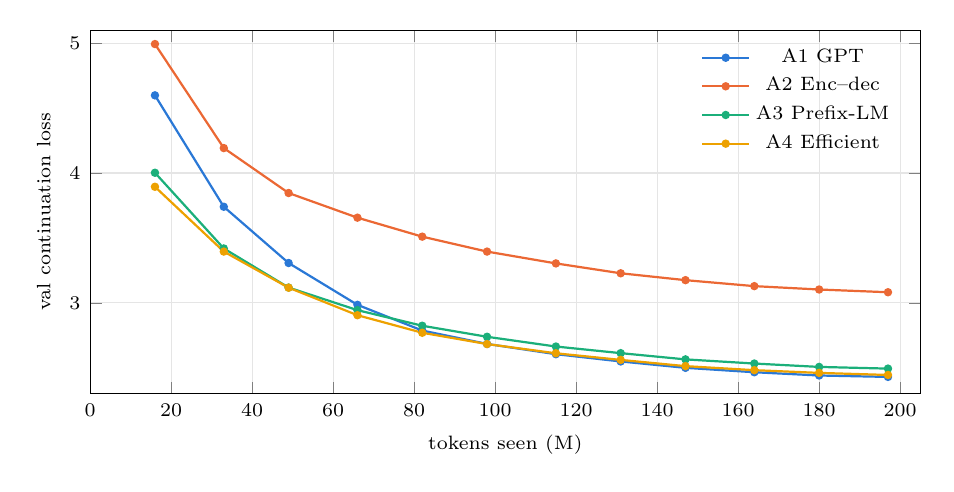
\begin{tikzpicture}
        \begin{axis}[
          width=\linewidth, height=6.2cm,
          xlabel={tokens seen (M)}, ylabel={val continuation loss},
          xmin=0, xmax=205, ymin=2.3, ymax=5.1,
          grid=major, grid style={black!10},
          tick label style={font=\scriptsize}, label style={font=\scriptsize},
          legend style={font=\scriptsize, draw=none, fill=none, at={(0.98,0.98)}, anchor=north east},
          every axis plot/.append style={thick, mark=*, mark size=1.1pt},
        ]
          \addplot[color=cA1] coordinates {(16,4.598)(33,3.740)(49,3.307)(66,2.985)(82,2.787)(98,2.684)(115,2.605)(131,2.549)(147,2.500)(164,2.466)(180,2.441)(197,2.430)};
          \addlegendentry{A1 GPT}
          \addplot[color=cA2] coordinates {(16,4.993)(33,4.192)(49,3.846)(66,3.656)(82,3.510)(98,3.395)(115,3.304)(131,3.228)(147,3.175)(164,3.129)(180,3.103)(197,3.082)};
          \addlegendentry{A2 Enc--dec}
          \addplot[color=cA3] coordinates {(16,4.002)(33,3.419)(49,3.118)(66,2.944)(82,2.824)(98,2.739)(115,2.664)(131,2.613)(147,2.565)(164,2.533)(180,2.507)(197,2.494)};
          \addlegendentry{A3 Prefix-LM}
          \addplot[color=cA4] coordinates {(16,3.894)(33,3.395)(49,3.117)(66,2.905)(82,2.770)(98,2.683)(115,2.612)(131,2.561)(147,2.513)(164,2.482)(180,2.461)(197,2.445)};
          \addlegendentry{A4 Efficient}
        \end{axis}
      \end{tikzpicture}
    \end{column}
    \begin{column}{0.38\textwidth}
      \footnotesize
      \begin{itemize}
        \item \textbf{A4 and A3 learn fastest early}: at 16M tokens A4 is 0.70 nats ahead of A1.
              RoPE/ALiBi and RMSNorm+SwiGLU speed up early learning.
        \item \textbf{A1 overtakes after about 100M tokens} and finishes best.
        \item \textbf{All curves still fall} in the last 16M tokens (A1 $-0.011$, A4 $-0.017$, A2 $-0.021$), even though the learning rate has already decayed to its floor.
        \item Budget: 196.6M tokens for 82M parameters is \textbf{2.4 tokens per parameter}, against the $\approx$20 that is compute-optimal (Chinchilla).
      \end{itemize}
    \end{column}
  \end{columns}
\end{frame}

\begin{frame}{Efficiency: the GPU is mostly idle}
  \begin{columns}[c]
    \begin{column}{0.52\textwidth}
      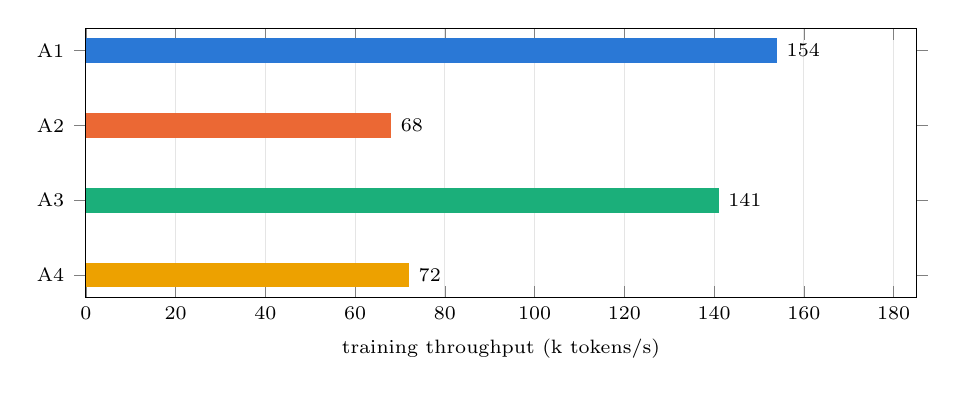
\begin{tikzpicture}
        \begin{axis}[
          xbar, width=\linewidth, height=5.0cm,
          xlabel={training throughput (k tokens/s)},
          symbolic y coords={A4,A3,A2,A1}, ytick={A4,A3,A2,A1},
          xmin=0, xmax=185, bar width=9pt,
          nodes near coords, nodes near coords style={font=\scriptsize},
          tick label style={font=\scriptsize}, label style={font=\scriptsize},
          major grid style={black!10}, xmajorgrids, bar shift=0pt,
        ]
          \addplot[fill=cA1, draw=none] coordinates {(154,A1)};
          \addplot[fill=cA2, draw=none] coordinates {(68,A2)};
          \addplot[fill=cA3, draw=none] coordinates {(141,A3)};
          \addplot[fill=cA4, draw=none] coordinates {(72,A4)};
        \end{axis}
      \end{tikzpicture}
    \end{column}
    \begin{column}{0.44\textwidth}
      \small
      \begin{tabular}{@{}lrrr@{}}
        \toprule
        Run & GPU util & peak alloc & energy\\
        \midrule
        A1 & 35\% & 6.8 GB & 0.093 kWh\\
        A2 & 14\% & 5.4 GB & 0.110 kWh\\
        A3 & 36\% & 7.0 GB & 0.097 kWh\\
        A4 & 29\% & 8.4 GB & 0.151 kWh\\
        \bottomrule
      \end{tabular}
      \vspace{2mm}
      \begin{itemize}
        \item The runs use \textbf{under 9 GB of a 141 GB card} and under 40\% of its compute.
        \item A4 is ``efficient'' on paper but trains at \textbf{half the speed} of A1. The sliding window is applied as a mask over full attention, so it saves no FLOPs, and A4 has 10 layers rather than 8.
        \item Faster training means more tokens per GPU-hour.
      \end{itemize}
    \end{column}
  \end{columns}
\end{frame}

\begin{frame}{What we learn from A1--A4}
  \begin{columns}[T]
    \begin{column}{0.49\textwidth}
      \begin{block}{Findings}
        \small
        \begin{enumerate}
          \item \textbf{Single-stack models win.} A2 splits its capacity: the decoder that writes the continuation has only 6 layers at $d{=}640$.
          \item \textbf{A4's modern components do not pay off at 200M tokens}, even with 25\% more depth. The early lead fades.
          \item \textbf{The models are undertrained} (2.4 tokens/parameter; curves still falling).
          \item \textbf{BERTScore is coarse.} A 0.65-nat gap (A2) costs 0.021 BERTScore, but a 0.06-nat gap (A1 vs A3) moves it by only 0.0015.
        \end{enumerate}
      \end{block}
    \end{column}
    \begin{column}{0.47\textwidth}
      \begin{alertblock}{Generation problems seen on the test set}
        \small
        \begin{itemize}
          \item Degenerate loops, for example ``\code{.l.l.l.l}'' in test ID 773, and repeated sentences.
          \item With \code{max\_new\_tokens}=256, 10 of 1000 continuations fell short of 128 words; 512 tokens left 1 short.
        \end{itemize}
      \end{alertblock}
      \begin{exampleblock}{So what?}
        \small
        The largest gains are likely from \textbf{more tokens}, \textbf{faster training} and \textbf{better decoding}, not from further architecture changes. A1 and A4 are the two candidates to scale.
      \end{exampleblock}
    \end{column}
  \end{columns}
\end{frame}

% =====================================================================
\section{Next experiments}

\begin{frame}{E1: train longer (the biggest lever)}
  \begin{columns}[T]
    \begin{column}{0.52\textwidth}
      \small
      \textbf{Question:} how much does loss keep falling with more tokens?
      \begin{itemize}
        \item Retrain A1 and A4 with \code{max\_steps} = 6k, 12k and 24k (0.4B, 0.8B and 1.6B tokens).
              The cosine schedule must be \emph{stretched}, not resumed: resuming at the $6\!\times\!10^{-5}$ floor would waste the extra tokens.
        \item Set \code{train\_tokens} to match so no data is repeated.
        \item Save intermediate checkpoints (every 2k steps) to use in E7.
      \end{itemize}
      \vspace{1mm}
\begin{semiverbatim}\scriptsize
python scripts/04\_train.py --config configs/a1\_gpt.yaml \textbackslash
  --set train.max\_steps=12000 data.train\_tokens=800\_000\_000 \textbackslash
        run\_name=A1\_gpt\_12k
\end{semiverbatim}
    \end{column}
    \begin{column}{0.44\textwidth}
      \begin{block}{Read-out}
        \small Plot val loss and dev BERTScore against tokens on a log axis. Fit $L(D)=E+B/D^{\beta}$ and extrapolate to decide the final budget.
      \end{block}
      \begin{exampleblock}{Cost}
        \small A1 at 12k steps is about 1.6 GPU-h at today's speed, or well under 1 GPU-h after E2.
      \end{exampleblock}
      \begin{alertblock}{Hypothesis}
        \small A4's gated MLP and RoPE close the gap to A1, or overtake it, once data is no longer the bottleneck.
      \end{alertblock}
    \end{column}
  \end{columns}
\end{frame}

\begin{frame}{E2: make training faster before making it longer}
  \begin{columns}[T]
    \begin{column}{0.50\textwidth}
      \small
      \textbf{Question:} how much of the H200 can we actually use?
      \begin{itemize}
        \item \code{train.compile=true} (\code{torch.compile}).
        \item \code{micro\_batch\_size} 8$\to$32 with \code{grad\_accum\_steps} 8$\to$2. The tokens per step stay the same, so the results remain comparable.
        \item Use \code{scaled\_dot\_product\_attention} (Flash) for every layer. Give A4's window layers a real banded kernel (FlexAttention) instead of a dense mask.
        \item Profile the data loader: memory-mapped token bins, \code{pin\_memory}, more workers.
      \end{itemize}
    \end{column}
    \begin{column}{0.46\textwidth}
      \begin{block}{Read-out}
        \small Tokens/s, GPU utilisation and peak VRAM from \code{resources.csv}.
        Check that the loss curve \emph{does not change}: this is an engineering experiment, not a modelling one.
      \end{block}
      \begin{exampleblock}{Target}
        \small At least $2\times$ throughput for A1 and $3\times$ for A4, which makes E1 and E3 affordable.
      \end{exampleblock}
    \end{column}
  \end{columns}
\end{frame}

\begin{frame}{E3: which A4 component helps? (one-at-a-time ablation)}
  \small
  A1 and A4 differ in five ways at once, so we cannot tell which change helped early and which hurt late.
  Starting from A1, add one A4 component per run (same data, same 3000 steps):

  \vspace{2mm}
  \centering
  \begin{tabularx}{0.92\textwidth}{@{}llX@{}}
    \toprule
    Run & Change from A1 & What it isolates\\
    \midrule
    E3a & learned positions $\to$ RoPE & positional scheme (fast early learning?)\\
    E3b & LayerNorm $\to$ RMSNorm & normalisation (expected to be nearly neutral)\\
    E3c & GELU 3072 $\to$ SwiGLU 2048 & gated feed-forward at equal FLOPs\\
    E3d & 12 KV heads $\to$ 4 (GQA) & quality cost of the smaller KV cache\\
    E3e & full attention $\to$ window 256 + global every 3 & does local attention hurt long legal references?\\
    E3f & 8 layers $\to$ 10 layers at A1 width & depth versus the rest\\
    \bottomrule
  \end{tabularx}

  \vspace{2mm}
  \raggedright
  Read-out: final val loss and loss at 50M tokens. Keep the components that help at \emph{both} points in the scaled model.
  These are ablations of one design, not new architectures, so they count as analysis rather than towards the four-architecture requirement.
\end{frame}

\begin{frame}{E4: use the parameter budget}
  \begin{columns}[T]
    \begin{column}{0.52\textwidth}
      \small
      \textbf{Question:} at a fixed GPU-hour budget, is it better to have more parameters or more tokens?
      The rules allow up to \textbf{300M}; we use 82M.

      \vspace{2mm}
      \begin{tabular}{@{}lrrr@{}}
        \toprule
        Size & $d$ & layers & params\\
        \midrule
        S (current) & 768 & 8 & 82M\\
        M & 1024 & 12 & $\approx$185M\\
        L & 1024 & 20 & $\approx$286M\\
        \bottomrule
      \end{tabular}

      \vspace{2mm}
      Train each at 2--3 token budgets so every size has an iso-FLOP point (IsoFLOP curves, Chinchilla approach~3).
    \end{column}
    \begin{column}{0.44\textwidth}
      \begin{block}{Read-out}
        \small Val loss against FLOPs ($\approx 6ND$). Pick the size on the lower envelope for the final budget.
      \end{block}
      \begin{alertblock}{Watch}
        \small
        \begin{itemize}
          \item \code{enforce\_param\_budget} must stay on.
          \item Larger models slow down inference in Phases 2--7 and need a lower peak lr (for example $3\!\times\!10^{-4}$).
          \item Model size is a scaling study, not a new architecture.
        \end{itemize}
      \end{alertblock}
    \end{column}
  \end{columns}
\end{frame}

\begin{frame}{E5: decoding (cheap, and scored directly by BERTScore)}
  \begin{columns}[T]
    \begin{column}{0.52\textwidth}
      \small
      \textbf{Question:} which decoder gives the best dev BERTScore for a fixed checkpoint?
      Each point is one run of \code{05\_generate.py} + \code{06\_evaluate.py} on the 200 dev prompts (about 1 min on the H200).

      \vspace{1mm}
      \begin{itemize}
        \item Greedy, and greedy + repetition penalty 1.1 / 1.2 / 1.3.
        \item $\tau \in \{0.3, 0.5, 0.7, 0.8, 1.0\}$ $\times$ top-$p \in \{0.8, 0.9, 0.95\}$.
        \item Add \textbf{no-repeat $n$-gram} blocking ($n{=}3,4$) to remove loops like ``\code{.l.l.l}''.
        \item Try min-$p$ sampling and beam search (width 4) as extra baselines.
        \item Repeat the best 3 settings with 3 seeds to measure noise.
      \end{itemize}
    \end{column}
    \begin{column}{0.44\textwidth}
      \begin{block}{Why it matters}
        \small BERTScore and ROUGE reward text \emph{close to the reference}. Lower-entropy decoding usually scores higher than creative sampling, while greedy decoding without penalties loops.
      \end{block}
      \begin{exampleblock}{Also fix}
        \small Raise the default \code{max\_new\_tokens} to 512 and add a fallback when a sample still has fewer than 128 words, for example resampling that prompt with a different seed.
      \end{exampleblock}
    \end{column}
  \end{columns}
\end{frame}

\begin{frame}{E6: data, tokenizer and context}
  \footnotesize
  \begin{tabularx}{\textwidth}{@{}lXX@{}}
    \toprule
    Exp. & Controlled change & Read-out\\
    \midrule
    E6a Data mix & Drop one source at a time; judgment-only mix; acts 10\%$\to$0\% & val loss \emph{per source}, dev BERTScore\\
    E6b Match the test set & Estimate the source of each test prompt (acts vs judgments, SC vs HC) and match the training mix to it & dev BERTScore on a test-like dev set\\
    E6c Tokenizer & Legal BPE 16k / 32k / 48k vs GPT-2 BPE & tokens per word, val loss \emph{per word} (comparable across vocabularies)\\
    E6d Context & Block 512 / 1024 / 2048; how much of the prompt is kept at decode time & val loss, dev BERTScore, speed\\
    E6e Regularisation & Dropout 0.1 and more weight decay, but only once data is repeated (multi-epoch) & train--val gap\\
    \bottomrule
  \end{tabularx}

  \vspace{1mm}
  \begin{alertblock}{A trap to avoid}
    \small Different tokenizers produce different numbers of tokens for the same text, so compare loss \textbf{per word} (bits per word), not per token.
  \end{alertblock}
\end{frame}

\begin{frame}{E7: does lower perplexity mean better text?}
  \begin{columns}[T]
    \begin{column}{0.52\textwidth}
      \small
      This is the key question in the brief. We have only 4 points so far: A2 is clearly separated, but the other three are tied on BERTScore.
      \begin{itemize}
        \item Score \textbf{every intermediate checkpoint} from E1 (for example 6 checkpoints $\times$ 2 models) and every E3 and E4 run on the dev set, all with the \emph{same} decoder.
        \item Plot dev BERTScore / ROUGE-L against val loss and report Spearman $\rho$.
        \item Use bootstrap confidence intervals over the 200 dev prompts to show which differences are real.
        \item Grow the dev set to 500--1000 prompts if the intervals overlap.
      \end{itemize}
    \end{column}
    \begin{column}{0.44\textwidth}
      \begin{block}{Checkpoint selection}
        \small Compare \code{best.pt}, \code{last.pt} and an average of the last $k$ checkpoints (or an EMA of the weights). Averaging is free and often gains a little.
      \end{block}
      \begin{exampleblock}{Outcome}
        \small A decision rule for which run gets one of the limited Codabench submissions.
      \end{exampleblock}
    \end{column}
  \end{columns}
\end{frame}

\begin{frame}{E8: distillation into a compact student}
  \begin{columns}[T]
    \begin{column}{0.52\textwidth}
      \small
      \textbf{Question:} can a smaller model keep most of the teacher's quality?
      \begin{itemize}
        \item Teacher: the best scaled model from E1/E4.
        \item Student: an A4-style model at about 50M parameters (the minimum allowed), using \code{configs/distill\_efficient\_small.yaml}.
        \item Compare three students: from scratch; logit KD ($\tau{=}2$, $\alpha{=}0.5$); KD plus a sweep over $\alpha$.
        \item All three see the same tokens.
      \end{itemize}
    \end{column}
    \begin{column}{0.44\textwidth}
      \begin{block}{Read-out}
        \small Val loss, dev BERTScore, decoding tokens/s and VRAM. Report the share of the teacher's gain over the scratch student that KD recovers.
      \end{block}
      \begin{exampleblock}{Why now}
        \small KD is \textbf{mandatory} in Phases 2--7. Getting the pipeline right in Phase 1 costs one short run.
      \end{exampleblock}
    \end{column}
  \end{columns}
\end{frame}

% =====================================================================
\section{Plan}

\begin{frame}{Priorities and budget}
  \small
  \centering
  \begin{tabularx}{\textwidth}{@{}clXrc@{}}
    \toprule
    \# & Experiment & Why & GPU-h & Expected gain\\
    \midrule
    1 & E2 faster training & Makes every later run cheaper & 0.5 & none (enabler)\\
    2 & E5 decoding sweep & Directly moves the leaderboard metric; fixes loops & 0.5 & medium\\
    3 & E1 longer training (A1, A4) & Models are clearly undertrained & 3--6 & \textbf{high}\\
    4 & E7 perplexity vs BERTScore & The core analysis question; decides submissions & 0.5 & analysis\\
    5 & E3 A4 ablations & Explains A1 vs A4; picks final components & 2 & low--medium\\
    6 & E4 model size & Uses the unused 82M$\to$300M budget & 4--8 & medium--high\\
    7 & E6 data / tokenizer / context & Domain fit to the test prompts & 3 & medium\\
    8 & E8 distillation & Rehearsal for Phases 2--7 & 1--2 & compact model\\
    \bottomrule
  \end{tabularx}

  \vspace{3mm}
  \raggedright
  GPU-hours are estimates at today's throughput; E2 should roughly halve them.
  A2 is dropped from scaling: it trails by 0.65 nats and trains at 44\% of A1's speed.
\end{frame}

\begin{frame}{Summary}
  \begin{columns}[T]
    \begin{column}{0.49\textwidth}
      \begin{block}{Where we are}
        \small
        \begin{itemize}
          \item Best model: \textbf{A1 GPT}, val loss 2.430 (ppl 11.36), dev BERTScore 0.8364.
          \item A4 is close (2.445); A3 is next (2.494); A2 is well behind (3.082).
          \item A1, A3 and A4 are tied on dev BERTScore.
          \item Every run is undertrained and uses a fraction of the GPU.
        \end{itemize}
      \end{block}
    \end{column}
    \begin{column}{0.47\textwidth}
      \begin{exampleblock}{What next}
        \small
        \begin{enumerate}
          \item Speed up training (E2).
          \item Tune decoding (E5).
          \item Train A1 and A4 for 4--8$\times$ more tokens (E1), then scale the winner (E4).
          \item Tie val loss to BERTScore with confidence intervals (E7).
          \item Distil the final model (E8).
        \end{enumerate}
      \end{exampleblock}
    \end{column}
  \end{columns}
\end{frame}

\end{document}
